\documentclass[12pt]{beamer}
\usepackage[inline]{asymptote}
\usepackage{animate}
\usepackage{graphicx}
\usefonttheme[onlymath]{serif}
\usepackage{amsmath}
\renewcommand{\vec}[1]{\mathbf{#1}}
\newcommand{\grad}{\nabla}
\newcommand{\partiald}[2]{\frac{\partial {#1} }{\partial {#2}}}
\usepackage[english]{babel}
\usepackage[utf8x]{inputenc}
\usepackage{amsmath,amsfonts,amsthm,graphicx}
\usepackage{bm,amsmath,bbm,amsfonts,nicefrac,latexsym,amsmath,amsfonts,amsbsy,amscd,amsxtra,amsgen,amsopn,bbm,amsthm,amssymb,textcomp,graphicx,float,verbatim,physics,hyperref,tabu, marvosym}


%Information to be included in the title page:
\usepackage{bm}%fette Symbole(Vektoren)
\usepackage{nicefrac}
\usepackage{xcolor}
\usepackage{import}


\newcommand\Ccancel[2][black]{\renewcommand\CancelColor{\color{#1}}\xcancel{#2}}

\newcommand*{\HomePath}{} %Set Home Path

\graphicspath {{\HomePath Plots/}{Plots/}} %Set Plot Path
\subimport{}{commands.tex} %Import commands




\mode<presentation>
{
	\usetheme{Madrid}     
	\usecolortheme{}
	\usefonttheme{default}  
	\setbeamertemplate{navigation symbols}{}
	\setbeamertemplate{caption}[numbered]
	\setbeamercolor{block title}{bg=orange!70}
	
} 

\usepackage[english]{babel}
\usepackage[utf8x]{inputenc}


\title[Rossby Waves]{Rossby Waves}
\author{Manu, Sam, Philipp, Edward, Cathie}
\institute{University of Reading and Imperial College London}
\begin{document}
	
	\begin{frame}
	\titlepage
\end{frame}

\begin{frame}{Overview}

\begin{itemize}
	\item Introduce Rossby Waves and the Shallow Water Equations (SWE). (Manu)
	\item Potential Vorticity. (Philipp)
	\item Rossby Wave Model Derivation. (Sam)
	\item Linearisation. (Edward)
	\item Application of Rossby Waves. (Cathie)
\end{itemize}

\begin{figure}[H]
	\centering
	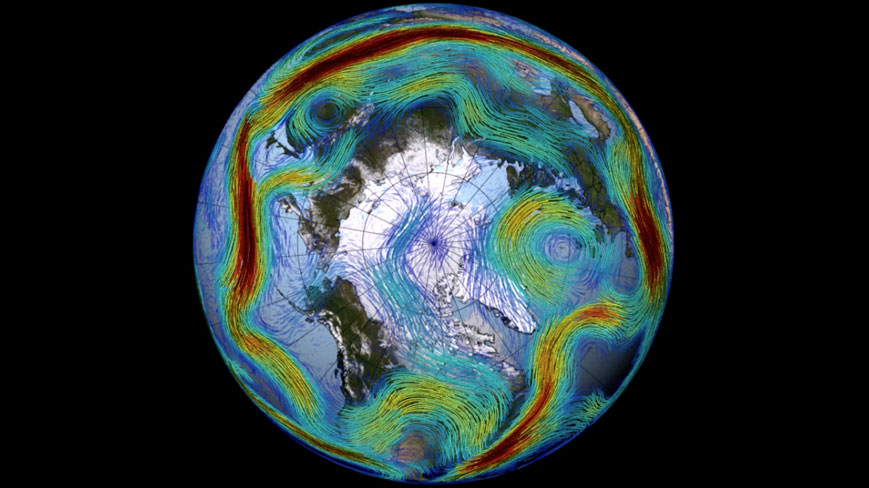
\includegraphics[width=0.5\linewidth]{Rossby_Wave.jpg}
\end{figure}   

\end{frame}


\begin{frame}{Introduction - Rossby Waves}

\begin{itemize}
\item Identified by Carl-Gustad Arvid Rossby.
\item Large meanders in high altitude winds.
\item Responsible for the weather at mid latitudes.
\item Caused by the Earth's rotation.
\item Two types of Rossby wave
\end{itemize}

\begin{table}[H]
\begin{center}
	\begin{tabular}{ |c|c|} 
		\hline
		\textbf{Barotropic} & \textbf{Baroclinic} \\
		\hline 
		Free wave & Forced wave \\  
		Progress eastward and fast moving & Slow moving ($cm/s$) \\
		Free travelling & Quasi stationary \\
		No significant vertical changes & Vertical changes \\
		\hline
	\end{tabular}
\end{center}
\end{table}

\begin{itemize}
\item Caused by conservation of \textbf{potential vorticity}.
\end{itemize}

\end{frame}

\begin{frame}{How do we get to the Rossby Waves?}

\begin{itemize}
\item Navier-Stokes \MVRightarrow  Shallow Water Equations (SWE) \MVRightarrow  Rossby Waves
\end{itemize}

\vspace{15pt}


The shallow water momentum equation -
\begin{equation}
\frac{\partial{\mathbf{u}}}{\partial{t}} + (\mathbf{u}\cdot\nabla)\mathbf{u} + f \textbf{z} \times \mathbf{u} = -g \nabla h \label{momentum_eq}
\end{equation}

The shallow water mass conservation - 

\begin{equation}
\frac{\partial h}{\partial t} + \nabla \cdot (h \mathbf{u}) = 0.\label{mass_conservation}
\end{equation}
\end{frame}
%\begin{frame}{What are the Shallow Water Equations?}
%
%\begin{itemize}
%\item A set of hyperbolic PDEs governing fluid flow in the oceans, coastal regions, rivers and channels.
%\item Consider the vertical length scale to be significantly smaller than the horizontal length scale.
%\item The SWE are derived from the Navier-Stokes equations.
%\item The Navier-Stokes equations are themselves derived from the equations for conservation of momentum (1) and the conservation of mass (2).
%\end{itemize}
%
%\vspace{-15pt}
%
%\begin{equation}   
%\rho(\frac{\partial{\mathbf{u}}}{\partial{t}} + \mathbf{u}.\nabla \mathbf{u}) = -\nabla p  + \mu \nabla^2\mathbf{u} + \rho \textbf{g},
%\end{equation}
%
%where $u=$ velocity, $p=$ pressure, $\rho=$ density and $\mu=$ viscosity.
%
%\begin{equation}
%\frac{\partial{\rho}}{\partial{t}} + (\nabla.\rho \mathbf{u}) = 0.
%\end{equation}
%
%\end{frame}
%
%
%\begin{frame}{Deriving the Shallow Water Equations}
%
%\begin{itemize}
%\item Derive the Navier-Stokes equations from the conservation laws (1) and (2).
%\item Specify boundary conditions for the Navier-Stokes equations for a water column.
%\item Use the boundary conditions to depth integrate the Navier-Stokes equations.
%\end{itemize}
%
%The Shallow Water Equation -
%\begin{equation}
%\frac{\partial{\mathbf{u}}}{\partial{t}} + \mathbf{u}.\nabla\mathbf{u} + f \textbf{z} \times \mathbf{u} = -g \nabla h
%\end{equation}
%
%\begin{itemize}
%\item Linearise the system of equations to perform analysis on.
%\end{itemize}
%
%\end{frame}
\begin{frame}
\frametitle{Vorticity Equation}
Rewrite SW equations in terms of \textit{relative vorticity} $\zeta=\nabla\times\bm{u}$
\vspace{0.3cm}
\begin{itemize}
	\item take the curl $\nabla \times \left(...\right)$
	\item $\pder{\zeta}{t}+\bm{u}\nabla(\zeta+f)=(\zeta+f)\nabla \bm{u}$
\end{itemize}
\vspace{0.5cm}
Inserting the mass conservation $\frac{\partial h}{\partial t}+\nabla\cdot(hu)=0$, we can restate the equations as
\begin{align}
\mder{q}{t}=0,\qquad q=\frac{\zeta+f}{h}\label{pv_conservation}.
\end{align}
\vspace{0.5cm}
The quantity $q$ is conserved, it is called the \textbf{potential vorticity}. 
\end{frame}
\begin{frame}
\frametitle{Potential Vorticity}
What does PV conservation imply? \hfill $\color{blue}\boxed{q=\frac{\zeta+f}{h}}$\\
\vspace{0.5cm}
In $f$-plane approximation, $f=f_0=$const. :
\vspace{0.2cm}
\begin{columns}
\begin{column}{0.48\textwidth}
	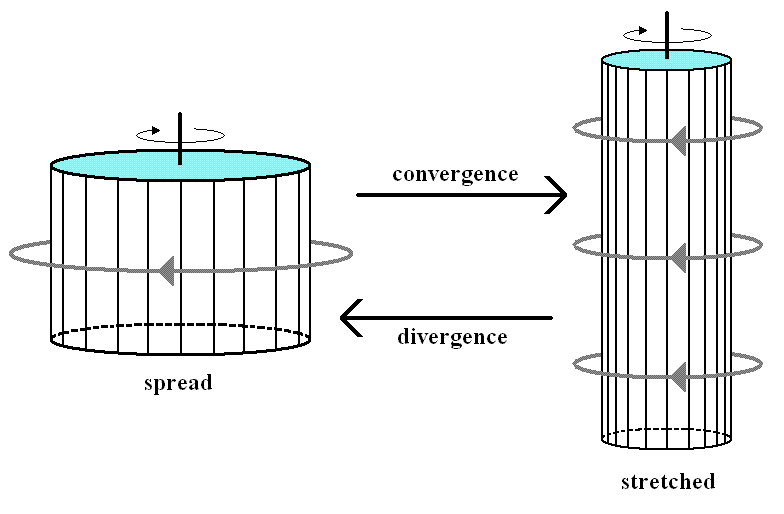
\includegraphics[width=\linewidth]{Potential_vorticity_conservation}
\end{column}
\begin{column}{0.48\textwidth}
	\begin{itemize}
		\item Change in $\zeta$ has to be compensated by change in height $h$
	\end{itemize}
\end{column}
\end{columns}
\end{frame}


\begin{frame}
\frametitle{Potential Vorticity}
In $\beta$-plane approximation $f=f_0+\beta y$ is not constant. \hfill $\color{blue}\boxed{q=\frac{\zeta+f}{h}}$\\
\vspace{0.5cm}
Fluid parcels can move north-/southward when changing vorticity $\zeta$.
\begin{columns}
\begin{column}{0.55\textwidth}
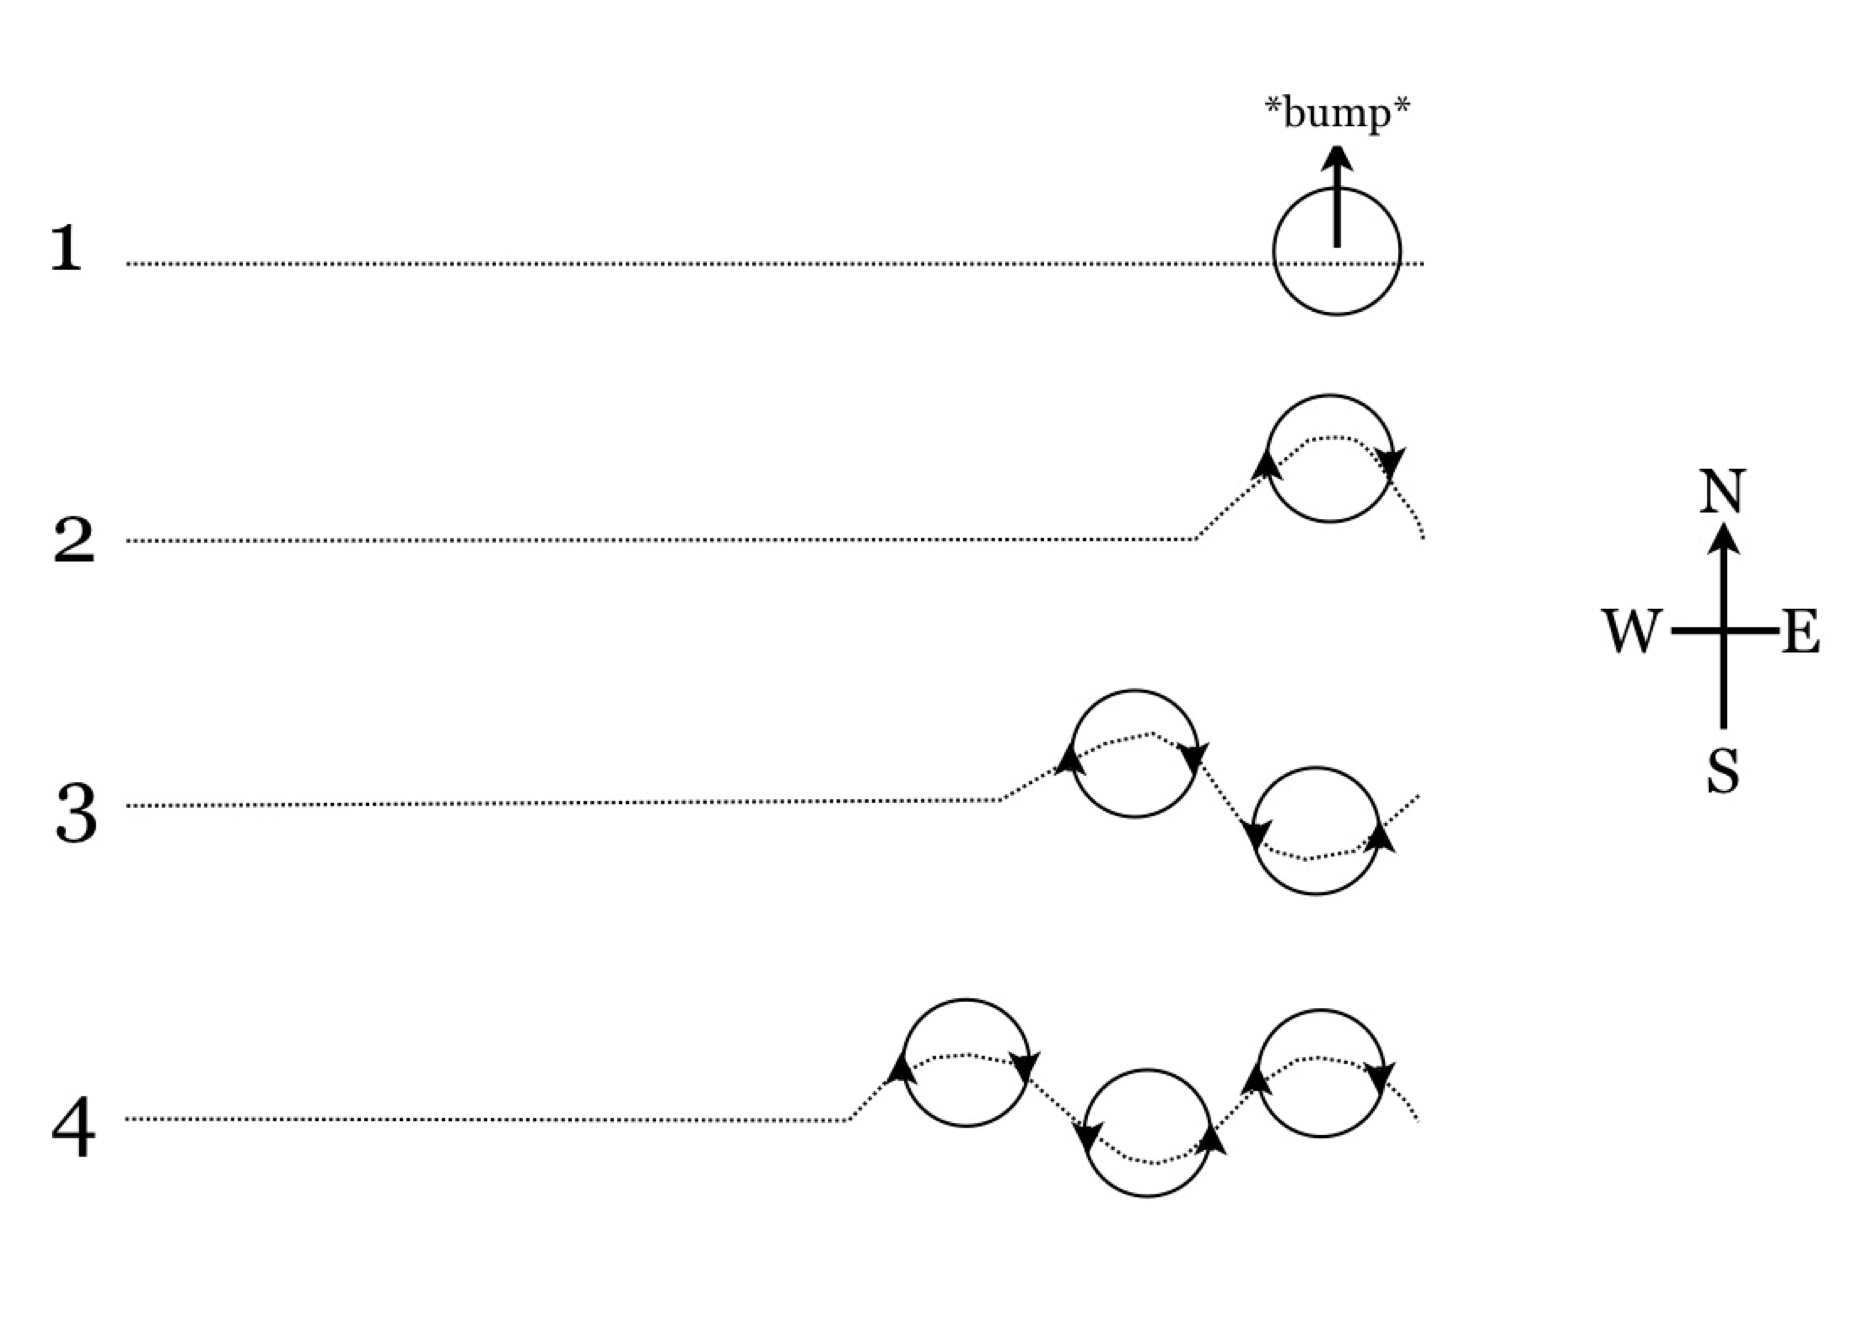
\includegraphics[width=\linewidth]{beta_plane}
\end{column}
\begin{column}{0.45\textwidth}
\begin{itemize}
	\item Additionally induce movement on neighboured fluid particles
\end{itemize}
\end{column}
\end{columns}
\end{frame}

\begin{frame}[fragile]
\frametitle{A simple model}

In order to obtain a model for the propogation of Rossby waves, we make the following simplifying assumptions:

 \begin{itemize}
\item The height of the free surface is fixed at $h=H$.
\item The Coriolis parameter varies linearly with latitude as $f=f_0+\beta y$ (beta plane approximation)
\end{itemize}

Then the potential vorticity equation \eqref{pv_conservation} reduces to

\[
\frac{D}{Dt}\left(\zeta+f_0+\beta y\right)=0
\]

which simplifies to

\[
\frac{D\zeta}{Dt}+\beta v=0
\]
\end{frame}


\begin{frame}[fragile]
\frametitle{A simple model}

Since $h$ is assumed constant, then the continuity equation \eqref{mass_conservation} implies that $\nabla \cdot \mathbf{u}=0$. Then there exists a stream function $\psi$ such that $\mathbf{u}=\left(-\frac{\partial \psi}{\partial y},\frac{\partial \psi}{\partial x}\right)$. By expanding the material derivative and writing $u$ and $v$ in terms of $\psi$, we get 

\[
\frac{\partial \zeta}{\partial t}-\frac{\partial \psi}{\partial y}\frac{\partial \zeta}{\partial x}+\frac{\partial \psi}{\partial x}\frac{\partial \zeta}{\partial y}+\beta\frac{\partial \psi}{\partial x}=0
\]

Then using the fact that $\zeta=\nabla^2\psi$, we obtain an equation for $\psi$:

\begin{equation}
\frac{\partial \left(\nabla^2 \psi\right)}{\partial t}-\frac{\partial \psi}{\partial y}\frac{\partial \left(\nabla^2 \psi\right)}{\partial x}+\frac{\partial \psi}{\partial x}\frac{\partial \left(\nabla^2 \psi\right)}{\partial y}+\beta\frac{\partial \psi}{\partial x}=0 \label{streamfunc_evolution}
\end{equation}
\end{frame}


\begin{frame}[fragile]
\frametitle{Linearization}
We see that a steady uniform flow with velocity $\mathbf{u_0}=\left(U,0\right)$ and stream function $\psi_0=-Uy$ satisfies equation \eqref{streamfunc_evolution}. 

We now consider a small perturbation $\psi=\psi_0+\epsilon\psi_1+O\left(\epsilon^2\right)$. By substituting this into \eqref{streamfunc_evolution} and discarding higher order terms we obtain the following equation for $\psi_1$:

\[
\frac{\partial \left(\nabla^2 \psi_1\right)}{\partial t}+U\frac{\partial \left(\nabla^2 \psi_1\right)}{\partial x}+\beta\frac{\partial \psi_1}{\partial x}=0
\]

Next we make the ansatz that $\psi_1=\cos\left(kx+ly-\omega t\right)$. Substituting this into the above equation, we obtain the following dispersion relation:

\[
\omega=Uk-\frac{\beta k}{k^2+l^2}
\]

\end{frame}




\begin{frame}[fragile]
\frametitle{Plot}
\begin{minipage}[t][6cm]{\textwidth}
\centering
	\begin{asy}
	import animate;
	import graph;
	import contour;
	import palette;
	
	pen[] pal={

rgb(0,42,215),
rgb(0,43,214),
rgb(0,43,213),
rgb(0,44,212),
rgb(0,44,212),
rgb(0,45,211),
rgb(0,45,210),
rgb(0,46,209),
rgb(7,46,208),
rgb(13,47,207),
rgb(19,47,206),
rgb(23,48,205),
rgb(27,48,204),
rgb(30,49,203),
rgb(33,49,202),
rgb(35,50,201),
rgb(38,50,201),
rgb(40,51,200),
rgb(42,51,199),
rgb(44,52,198),
rgb(46,52,197),
rgb(47,53,196),
rgb(49,53,195),
rgb(51,54,194),
rgb(52,54,193),
rgb(54,55,192),
rgb(55,55,191),
rgb(56,56,191),
rgb(58,56,190),
rgb(59,57,189),
rgb(60,57,188),
rgb(61,57,187),
rgb(62,58,186),
rgb(64,58,185),
rgb(65,59,184),
rgb(66,59,183),
rgb(67,60,182),
rgb(68,60,181),
rgb(69,61,181),
rgb(69,61,180),
rgb(70,62,179),
rgb(71,62,178),
rgb(72,63,177),
rgb(73,63,176),
rgb(74,64,175),
rgb(74,64,174),
rgb(75,64,173),
rgb(76,65,172),
rgb(77,65,172),
rgb(77,66,171),
rgb(78,66,170),
rgb(79,67,169),
rgb(79,67,168),
rgb(80,68,167),
rgb(81,68,166),
rgb(81,69,165),
rgb(82,69,164),
rgb(82,70,163),
rgb(83,70,163),
rgb(84,70,162),
rgb(84,71,161),
rgb(85,71,160),
rgb(85,72,159),
rgb(86,72,158),
rgb(86,73,157),
rgb(87,73,156),
rgb(87,74,155),
rgb(88,74,155),
rgb(88,74,154),
rgb(88,75,153),
rgb(89,75,152),
rgb(89,76,151),
rgb(90,76,150),
rgb(90,77,149),
rgb(91,77,148),
rgb(91,78,147),
rgb(91,78,146),
rgb(92,78,146),
rgb(92,79,145),
rgb(92,79,144),
rgb(93,80,143),
rgb(93,80,142),
rgb(93,81,141),
rgb(94,81,140),
rgb(94,82,139),
rgb(94,82,138),
rgb(94,82,138),
rgb(95,83,137),
rgb(95,83,136),
rgb(95,84,135),
rgb(96,84,134),
rgb(96,85,133),
rgb(96,85,132),
rgb(96,86,131),
rgb(96,86,130),
rgb(97,86,130),
rgb(97,87,129),
rgb(97,87,128),
rgb(97,88,127),
rgb(98,88,126),
rgb(98,89,125),
rgb(98,89,124),
rgb(98,89,123),
rgb(98,90,122),
rgb(98,90,122),
rgb(99,91,121),
rgb(99,91,120),
rgb(99,92,119),
rgb(99,92,118),
rgb(99,92,117),
rgb(99,93,116),
rgb(99,93,115),
rgb(99,94,114),
rgb(99,94,113),
rgb(100,95,113),
rgb(100,95,112),
rgb(100,95,111),
rgb(100,96,110),
rgb(100,96,109),
rgb(100,97,108),
rgb(100,97,107),
rgb(100,98,106),
rgb(100,98,105),
rgb(100,98,104),
rgb(100,99,103),
rgb(100,99,103),
rgb(100,100,102),
rgb(100,100,101),
rgb(101,100,100),
rgb(103,100,99),
rgb(105,100,99),
rgb(106,100,98),
rgb(108,100,97),
rgb(110,100,97),
rgb(111,99,96),
rgb(113,99,96),
rgb(114,99,95),
rgb(116,99,94),
rgb(117,99,94),
rgb(119,99,93),
rgb(120,99,92),
rgb(122,98,92),
rgb(123,98,91),
rgb(125,98,91),
rgb(126,98,90),
rgb(128,98,89),
rgb(129,98,89),
rgb(131,97,88),
rgb(132,97,87),
rgb(134,97,87),
rgb(135,97,86),
rgb(136,97,86),
rgb(138,96,85),
rgb(139,96,84),
rgb(140,96,84),
rgb(142,96,83),
rgb(143,96,82),
rgb(144,95,82),
rgb(146,95,81),
rgb(147,95,81),
rgb(148,95,80),
rgb(150,94,79),
rgb(151,94,79),
rgb(152,94,78),
rgb(154,94,77),
rgb(155,93,77),
rgb(156,93,76),
rgb(158,93,75),
rgb(159,93,75),
rgb(160,92,74),
rgb(161,92,73),
rgb(163,92,73),
rgb(164,91,72),
rgb(165,91,72),
rgb(166,91,71),
rgb(168,91,70),
rgb(169,90,70),
rgb(170,90,69),
rgb(171,90,68),
rgb(173,89,68),
rgb(174,89,67),
rgb(175,89,66),
rgb(176,88,66),
rgb(177,88,65),
rgb(179,88,64),
rgb(180,87,64),
rgb(181,87,63),
rgb(182,86,62),
rgb(183,86,62),
rgb(185,86,61),
rgb(186,85,60),
rgb(187,85,60),
rgb(188,84,59),
rgb(189,84,58),
rgb(191,84,58),
rgb(192,83,57),
rgb(193,83,56),
rgb(194,82,56),
rgb(195,82,55),
rgb(197,81,54),
rgb(198,81,53),
rgb(199,80,53),
rgb(200,80,52),
rgb(201,79,51),
rgb(202,79,51),
rgb(204,78,50),
rgb(205,78,49),
rgb(206,77,48),
rgb(207,77,48),
rgb(208,76,47),
rgb(209,76,46),
rgb(210,75,46),
rgb(212,74,45),
rgb(213,74,44),
rgb(214,73,43),
rgb(215,73,43),
rgb(216,72,42),
rgb(217,71,41),
rgb(218,71,40),
rgb(220,70,39),
rgb(221,69,39),
rgb(222,69,38),
rgb(223,68,37),
rgb(224,67,36),
rgb(225,66,35),
rgb(226,65,35),
rgb(228,65,34),
rgb(229,64,33),
rgb(230,63,32),
rgb(231,62,31),
rgb(232,61,30),
rgb(233,60,29),
rgb(234,59,28),
rgb(235,58,27),
rgb(237,58,27),
rgb(238,56,26),
rgb(239,55,25),
rgb(240,54,24),
rgb(241,53,22),
rgb(242,52,21),
rgb(243,51,20),
rgb(244,50,19),
rgb(246,48,18),
rgb(247,47,17),
rgb(248,46,15),
rgb(249,44,14),
rgb(250,43,13),
rgb(251,41,11),
rgb(252,40,9),
rgb(253,38,8),
rgb(255,36,6),
rgb(255,34,5),
rgb(255,32,3),
rgb(255,30,1),
rgb(255,27,0),
rgb(255,25,0)
	};
	
	real m=0.15;
	real k=6;
	real U=1.0;
	real beta=25.0;
	real w=U*k-beta/k;

real width=2;
real height=1;

pair[] tracer_positions;
	for(int i=-80;i<40;++i)
	for(int j=-5;j<25;++j)
	{
	tracer_positions.push((i*width/40.0,j*height/20.0));
	}

	picture getframe(real t)
	{
	picture frame;
	size(frame,10cm);
	

	real streamfunc(real x, real y)
	{
	return -U*y+m*cos(k*x-w*t);
	}
	
	real vorticity(real x,real y)
	{
	return -k*k*m*cos(k*x-w*t);
	}

	path velocity(pair z)
	{
	return (0,0)--(U,-m*k*sin(k*z.x-w*t));
	}

	void draw_tracer(pair pos_0)
	{
	pair pos=(U*t+pos_0.x,(m/U)*(cos((k*U-w)*t+k*pos_0.x)-cos(k*pos_0.x))+pos_0.y);
		if(pos.x>0&&pos.x<width&&pos.y>0&&pos.y<height)
		{
		fill(frame,circle(pos,0.005));
		}
	}
	image(frame,vorticity,Automatic,(0,0),(width,height),nx=256,ny=1,pal);
	draw(frame,contour(streamfunc,(0,0),(width,height),uniform(-1.5,1.5,30)));

		for(int i=0;i<tracer_positions.length;++i)
		{
		draw_tracer(tracer_positions[i]);
		}

	//add(frame,vectorfield(velocity,(0,0),(width,height),nx=18,ny=9));
	xaxis(frame,"x",xmin=0,xmax=width+0.1,arrow=EndArrow);
	yaxis(frame,"y",ymin=0,ymax=height+0.1,arrow=EndArrow);
	return frame;
	}

	animation A=animation("Rossby waves");
		for(int i=0;i<200;++i)
		{
		write(i);
		A.add(getframe(i*(2pi/(w*200.0))));
		}
	label(A.pdf("autoplay,loop"));
	\end{asy} 
\end{minipage}

A plot of the solution. The dots move with the flow and the black lines represent streamlines of the velocity field, obtained by plotting level sets of the stream function $\psi=-Uy+\cos(kx-wt)$. The colors indicate vorticity - red for positive and blue for negative.

\end{frame}

\begin{frame}
\frametitle{Quasi stationary synoptic Rossby waves high amplitude during weather events }
\framesubtitle{by Petoukhov, Rahmstorf, Pteri and Schellnhuber 2013}
\begin{itemize}
	\item Investigated physical model of quasi resonance effect.
	\item Forced wave trapping a free wave.
	\item Amplification of pressure system.
	\item Extreme weather results.
\end{itemize}
\centering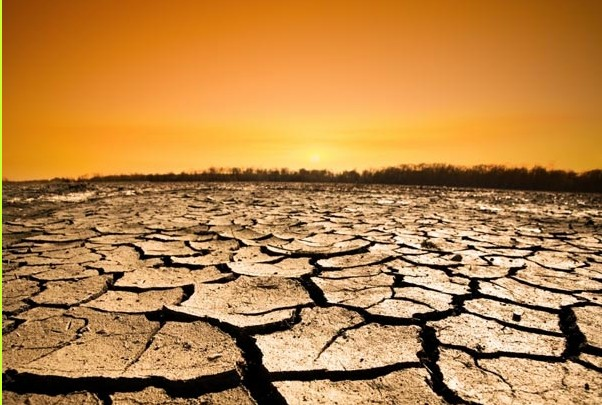
\includegraphics[height=0.4\textheight]{drought}

\end{frame}
\begin{frame}
\frametitle{Amplified mid-latitude planetary waves favour particular regional weather extremes}
\framesubtitle{ 
by Screen and Simmonds }
\begin{itemize}
\item Looked at distribution of quasi resonance events.
\item Examined links between temperature and precipitation anomalies and abnormal quasi stationary wave amplitude from 1979 to 2012.

\end{itemize}
\centering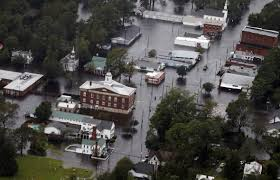
\includegraphics[height=0.4\textheight]{flood}
\end{frame}

\begin{frame}
\frametitle{40 most extreme temperature and precipitation events in the mid latitudes between 1979 and 2012.}
\centering
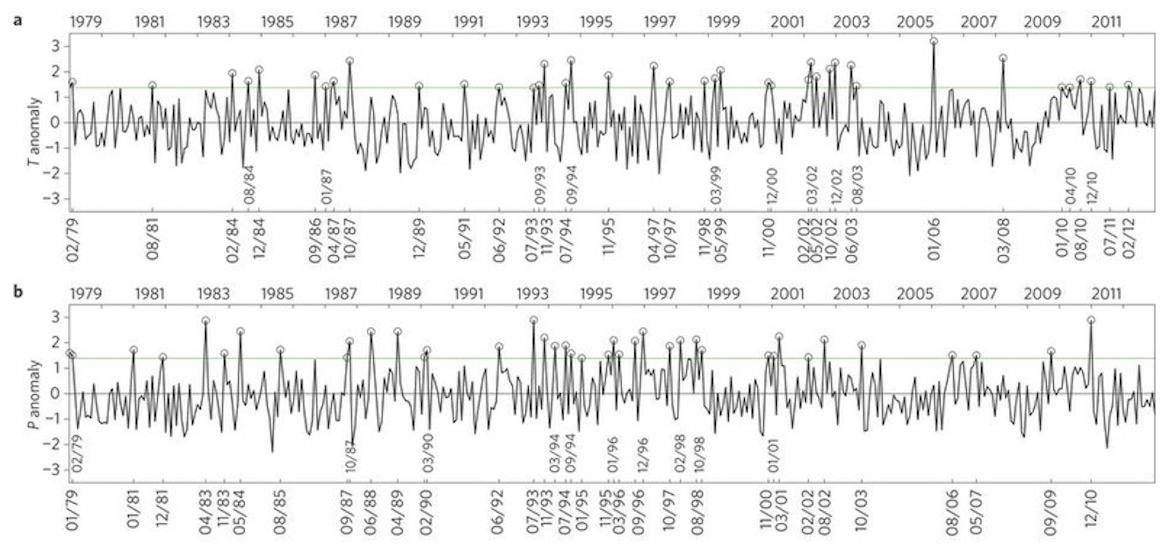
\includegraphics[scale=0.53]{Cathie1}


\end{frame}
\begin{frame}
\frametitle{Anomalies: Prolonged periods over a large area}
\begin{tabular}{c c}
\Large{Temperature}&\vspace{5pt}\\

\large{Positive: abnormally high}	&	\large{Negative: abnormally low}\vspace{20pt}\\

\Large{Precipitation}&\vspace{5pt}\\
\large{Positive: abnormally wet} &		\large{Negative: abnormally dry}\\
\end{tabular}
\end{frame}
\begin{frame}
\frametitle{Mid latitude regions of the Northern hemisphere examined}
\centering
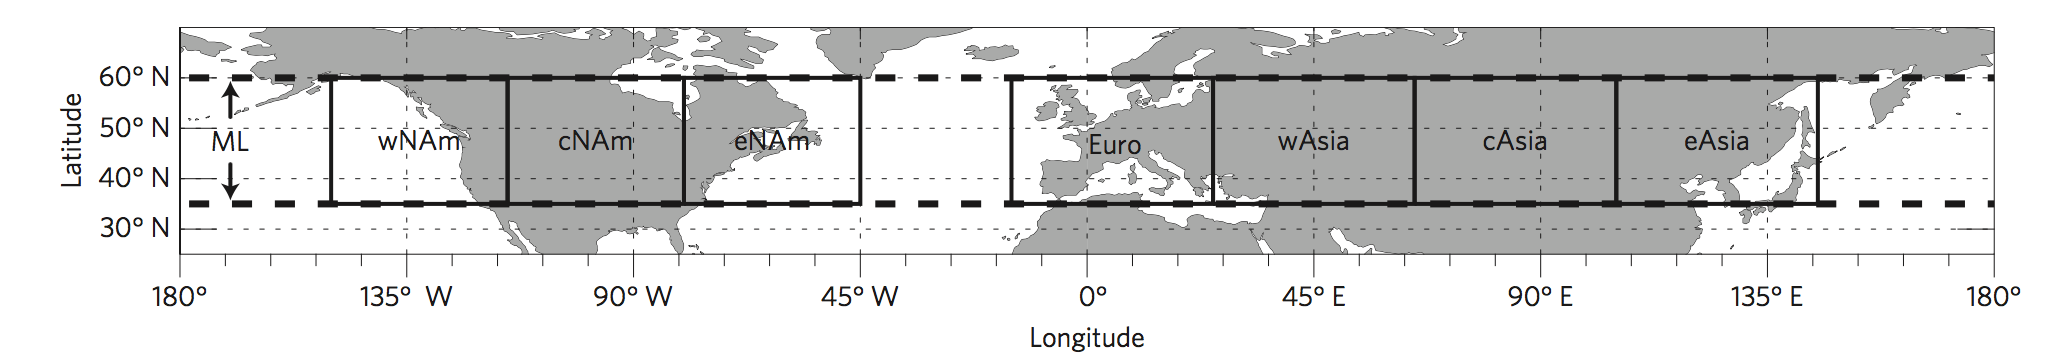
\includegraphics[scale=0.3]{Cathie2}
\end{frame}
\begin{frame}
\frametitle{Charts to show the normalized amplitude anomalies for each extreme temperature event, in order of severity of weather, taking the most extreme events on the left.}
\centering
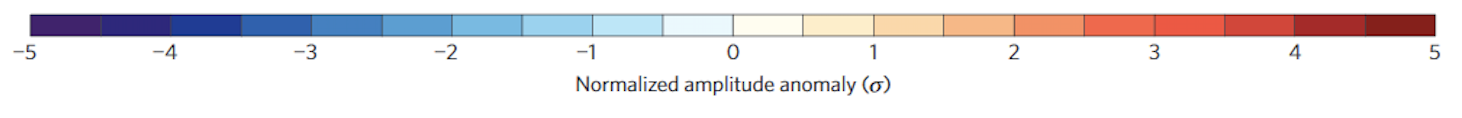
\includegraphics[scale=0.4]{Cathie4}
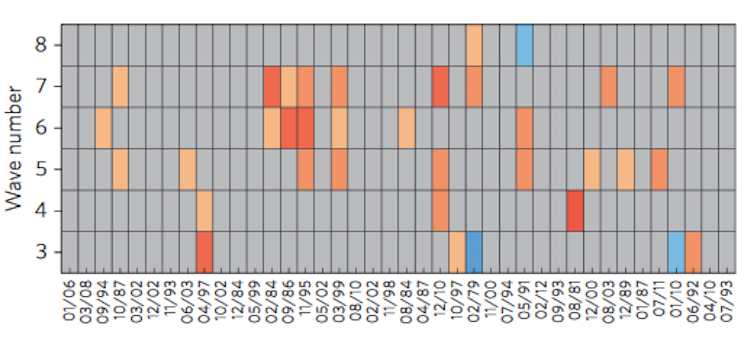
\includegraphics[scale=0.7]{Cathie5}
\end{frame}
\begin{frame}
\frametitle{Charts to show the normalized amplitude anomalies for each extreme precipitation event, in order of severity of weather, taking the most extreme events on the left.}
\centering
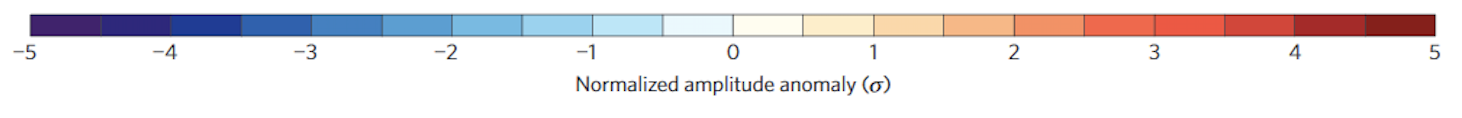
\includegraphics[scale=0.4]{Cathie4}
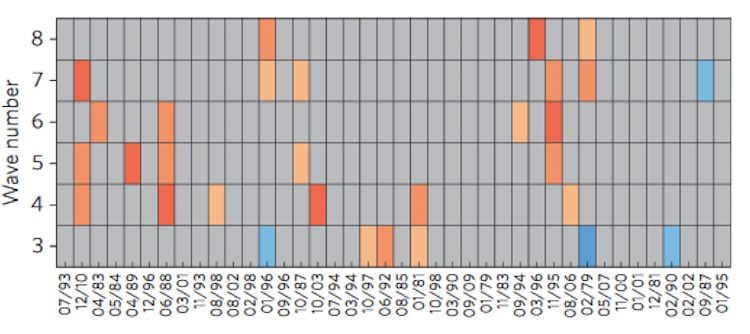
\includegraphics[scale=0.7]{Cathie6}
\end{frame}
\begin{frame}
\frametitle{Distributions comparing observed anomalies with results expected from climatology.}
\centering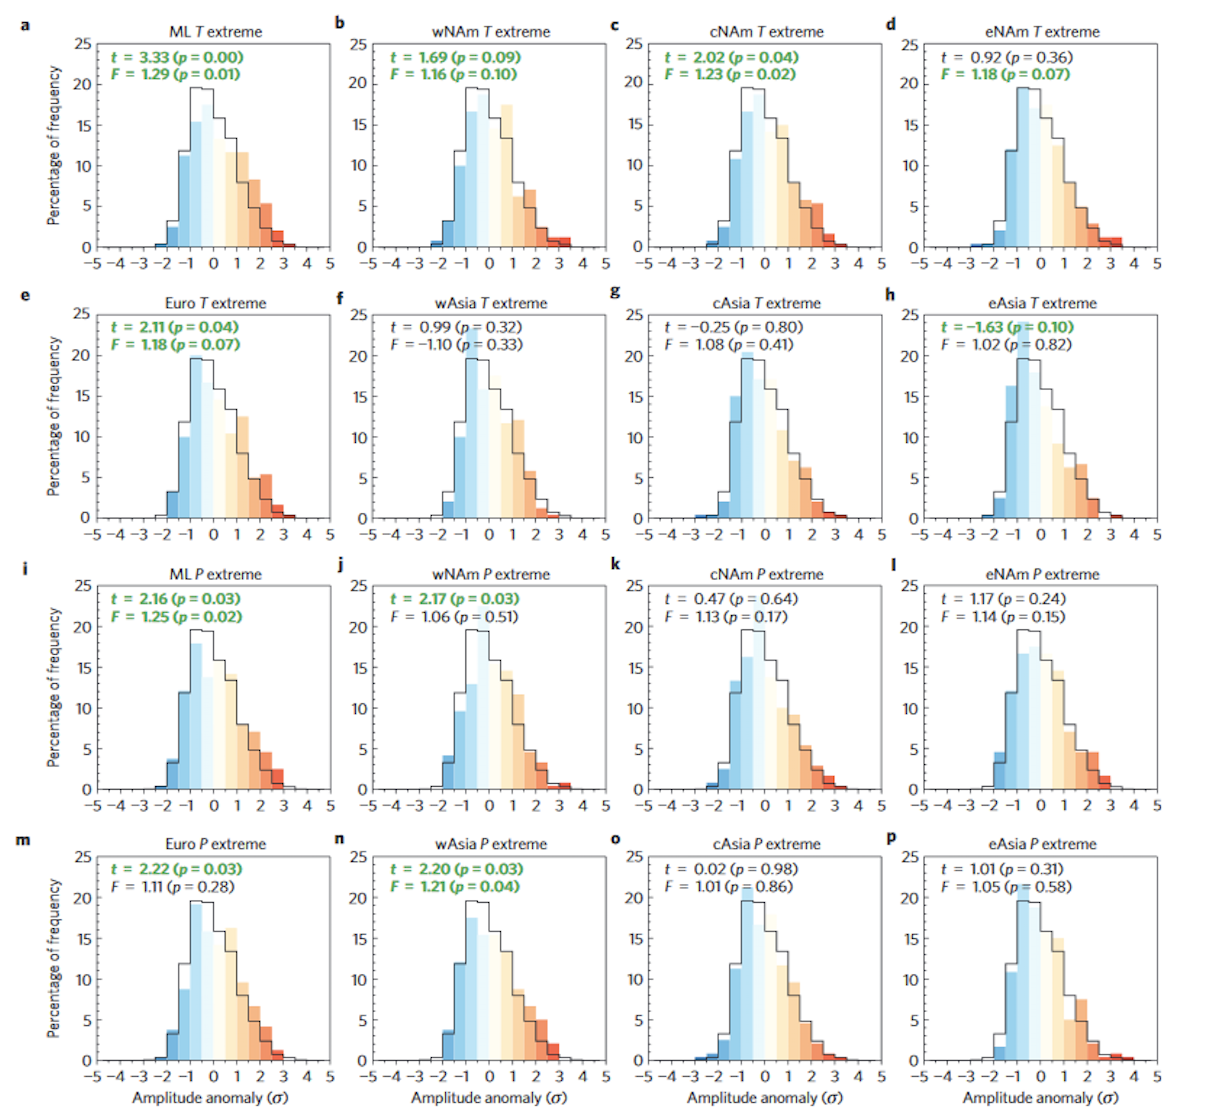
\includegraphics[scale=0.35]{Cathie7}
\end{frame}
\begin{frame}
\frametitle{Future Forecast}
\centering
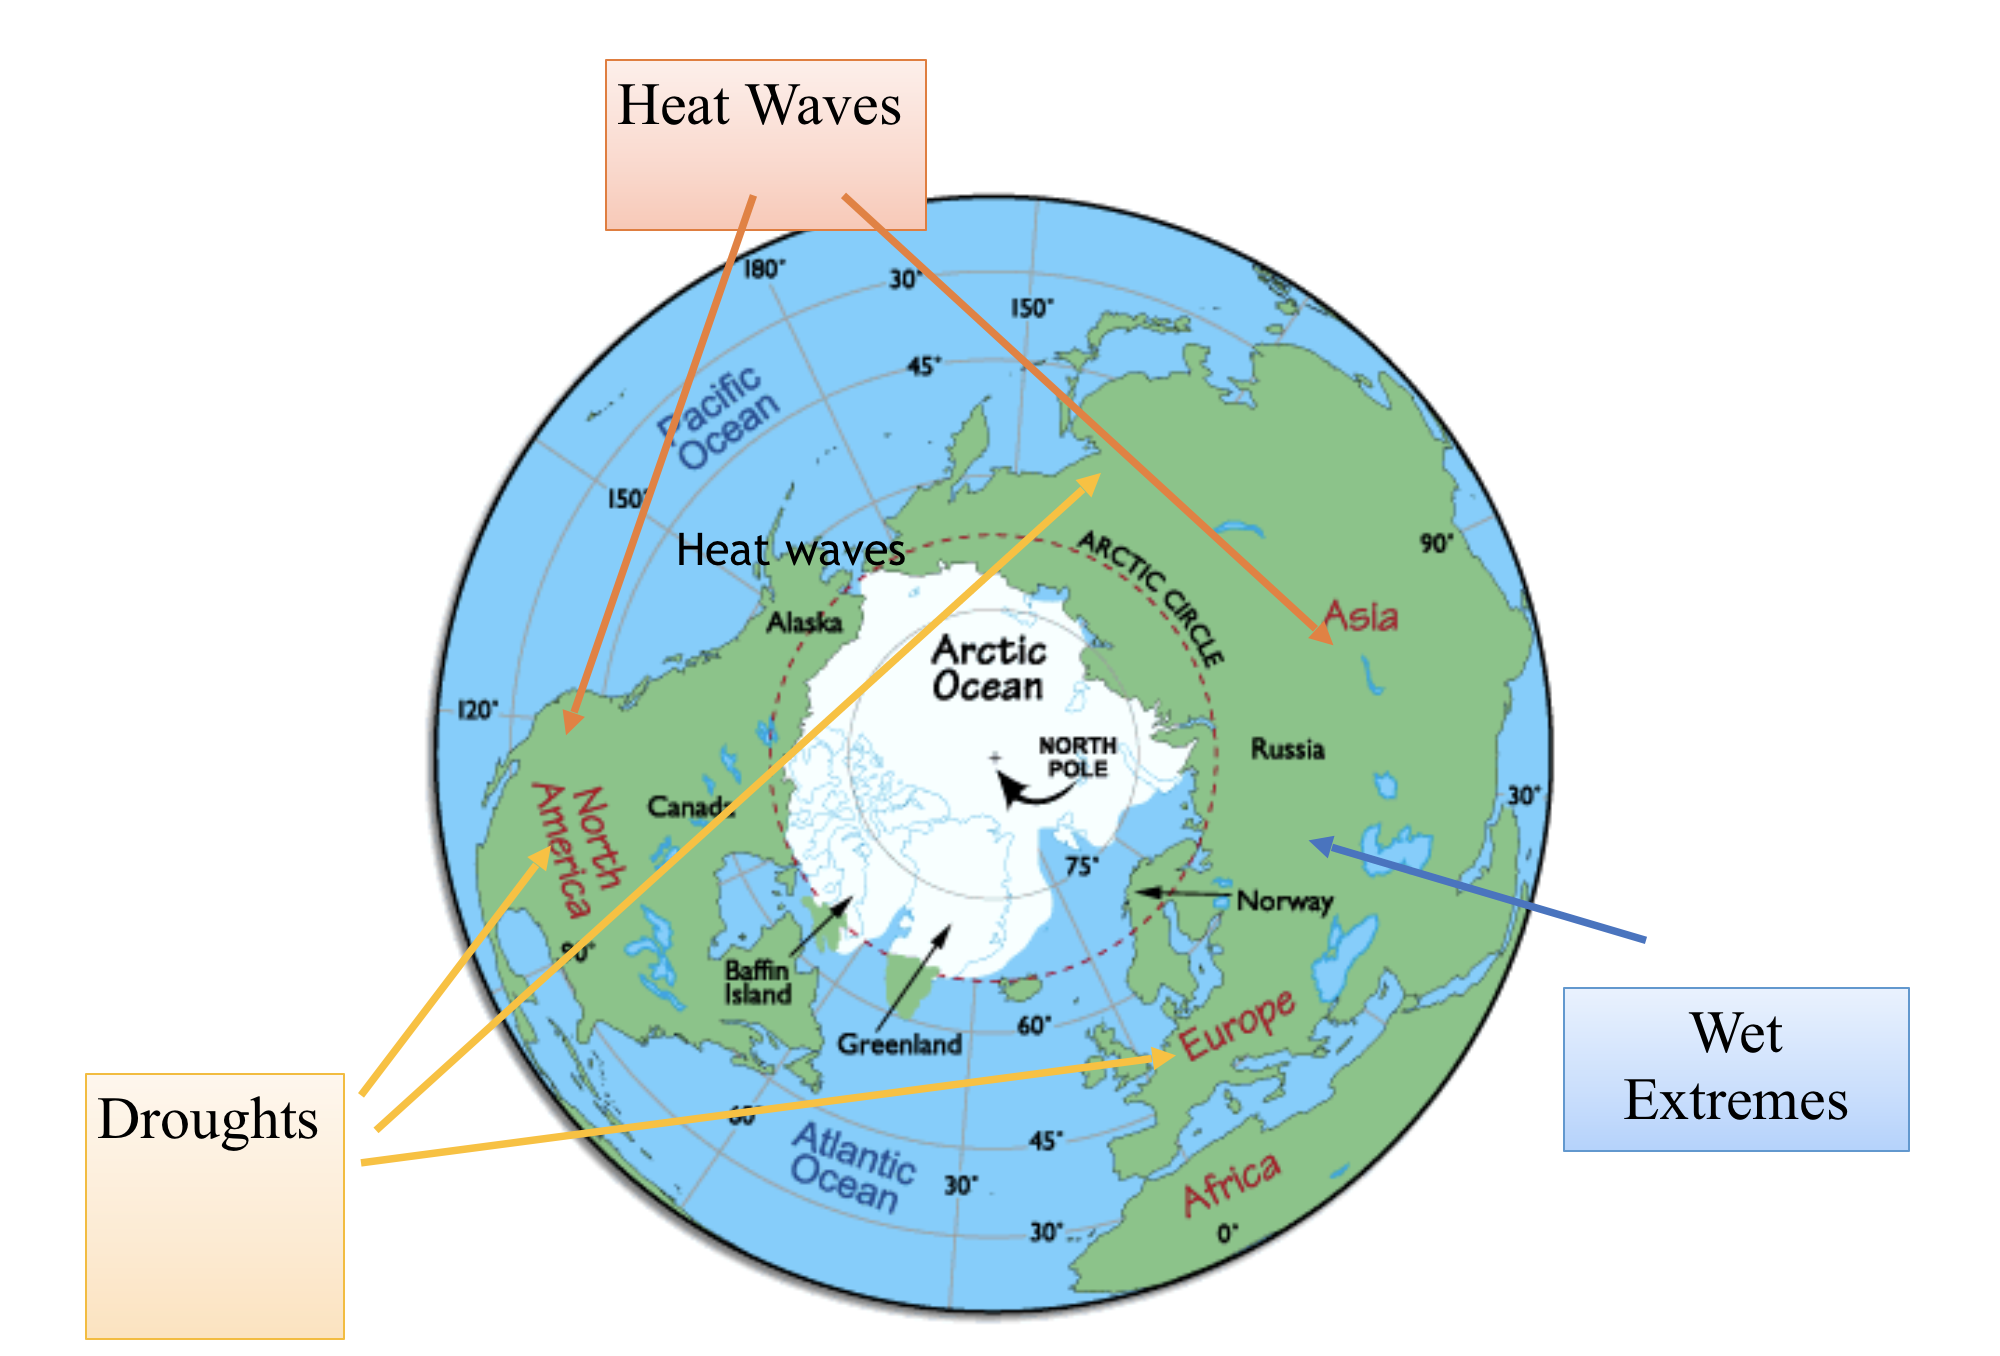
\includegraphics[scale=0.3]{Cathie8}


\end{frame}
\end{document}
